\documentclass{jsarticle}
\usepackage[top=20truemm,bottom=20truemm,left=25truemm,right=25truemm]{geometry}
\usepackage{amsmath,ascmac,url,amsfonts,bm,here,algorithmic,algorithm,amsthm,color}
\usepackage[dvipdfmx]{graphicx}
\newcommand{\argmax}{\mathop{\rm argmax}\limits}
\newcommand{\argmin}{\mathop{\rm argmin}\limits} 
\newcommand{\expect}{\mathbb{E}} 
\newcommand{\trans}[1]{#1^{\top}}
\newcommand{\pdif}[2]{\frac{\partial#1}{\partial#2}}
\newcommand{\odif}[2]{\frac{\rm{d}#1}{\rm{d}#2}}
\makeatletter
  \def\@maketitle{
  \newpage\null
  \vskip 2em
    \mbox{}\hfill
    \begin{flushleft}
    \textbf{制御システム論分野研究会資料}
    \end{flushleft}
    \begin{flushright}
    {\lineskip .5em
      \begin{tabular}[t]{c}
        \@date \\
        \@author
      \end{tabular}\par}
        \end{flushright}
  \begin{center}
  \let\footnote\thanks
    {\LARGE \@title \par}
    \vskip 1.5em
  \end{center}
    \vskip 1em
  \par}
\makeatother
\title{\large{\bf{進捗報告 8.15}}}
\author{M2 竹内 維吹}
%\date{Jul. 7, 2020}
\date{\today}
\begin{document}
\maketitle


\section{問題設定(作成中)}
以下のような入力アフィン系システムを考える.
\begin{equation}
	\dot{s}=f(s)+g(s)a \label{true_dynamics}
\end{equation}
ここで,~$s_t, a_t$はそれぞれ状態ベクトル, 入力ベクトルである.\par
さらに, 図1のようなシステム(\ref{true_dynamics})に対するイベント駆動型制御を考える.
\begin{figure}[h]
	\centering
 	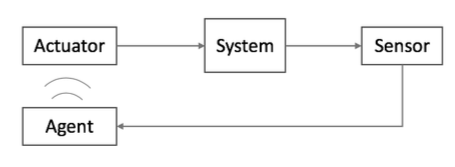
\includegraphics[width=8cm]{event.png}
 	\caption{イベント駆動型制御}
\end{figure}\\
ここではエージェントの制御則$\pi(s)$を設計するとし, $\pi(s)$はシステムに加えるべき入力信号$a$と, それを送信するかどうかを決定する2値変数$c~(c = 1 ならば送信)$で構成されるとする.つまり
\begin{equation}
	\pi(\cdot) = [~a, c~]^{\top}
\end{equation}
であるとする. このようなイベント駆動型制御に対して, 以下の条件を満たす最適イベント駆動型制御則$\pi^{*}(\cdot)$を導出する問題を考える.
\begin{align}
	\pi^{*}(\cdot) &= \argmax_{\pi}\expect_{s_0 \sim d_0}\left[V^{\pi} (s_0)\right] \label{optimal_policy}\\
	V^{\pi} (s_0) &=\sum_{t=0}^{\infty}(-s_t^{\top}Qs_t - \pi^{\top}(s_t)R\pi(s_t) - \lambda\gamma_t) \label{V}
\end{align}
ここで,~$\gamma_t$は時刻$t$においてエージェントがアクチュエータと通信を行ったかを表す2値変数である.また, $Q,R,\gamma$はそれぞれ正定値, 半正定値, 正のハイパーパラメータであり, $d_0$は初期状態を与える確率分布である.式(\ref{V})より, 「最小限の入力エネルギーで」かつ「最小限の通信回数で」「状態$s$を0に素早く漸近させる」と$V$が最大化される.\par
さて, システム(\ref{true_dynamics})が未知であるという設定のもとで, 実環境とのインタラクションによってデータ組$(s_t, a_t, r_t, s_{t+1})$を収集し, それらを活用することで上記の問題を解いていたのは\cite{event}である.\par
本研究ではさらに一歩踏み込んで, データ収集の実環境とのインタラクションの際に状態制約
\begin{equation}
	s\in C, C\subset S \label{constraint}
\end{equation}
を全時刻において満たしながら$\pi^{*}(\cdot)$を求める問題を考える.ただし, 式(\ref{optimal_policy})における$d_0$は$\textrm{support}(d_0)\subset C$を満たすとする.また, $S$は実環境において考えられうる全状態の集合であるとする.\par
\color{red}(現状, 上記の問題を解くことが研究の目標であると考えています.ただ, この先どのような仮定を置くかはまだ考えられていません. )

\color{black}
\section{DDPGとCBFを用いた解法}
システム(\ref{true_dynamics})に対して, 関数$h(s)$が以下の式を満たすならば,~$h(s)$は制御バリア関数(CBF)と呼ばれる.
\begin{equation}
	\sup_{a\in A}\left\{\pdif{h}{s}(f(s)+g(s)a)+K(h(s))\right\} \geq 0 \label{CBF}
\end{equation}
ただし, $K(s)$はクラスK関数である.\par
さて, 式(\ref{constraint})における状態制約$C$が
\begin{equation}
	C = \left\{s \in S~|~h(s)\geq 0\right\}
\end{equation}
として与えられているとする. このとき$h(s)$が制御バリア関数であるならば, 状態$s\in C$に対して次の時刻における状態$s^{\prime}$が$s^{\prime}\in C$を満たすようにする入力が存在することを保証する. そのような入力集合は現時刻での状態$s$に依存し,
\begin{equation}
	U(s) = \left\{a \in A~|~\pdif{h}{s}(f(s)+g(s)a)+K(h(s))\geq 0\right\}, \forall s\in C
\end{equation}
としてその集合を与える.\par
さて, DDPGなどの方策on型の強化学習では, 制御則$\pi(\cdot)$を用いて実環境とインタラクションを行い, データを収集・利活用することで, より$V^{\pi}$を大きくできるような制御則$\pi^{\prime}(\cdot)$を模索する.その過程で制御入力$\pi(s)$が$\pi(s)\notin U(s)$となるならば, 次時刻において状態制約$C$を満たさない状態に遷移してしまう.それを避けるため, $\pi(s)\notin U(s)$となった各時刻では, $\pi(s)$ではなく,~$\pi(s)$に最も近い$U(s)$の元を用いてインタラクションを行う手法を考えてみる.

\section{倒立振子による実験}
倒立時の振子の角度を$\theta=0$とし, 加えられる入力が$A=[-10\textrm{N}\cdot\textrm{m},10\textrm{N}\cdot\textrm{m}]$と制限されるような倒立振子を考える.この倒立振子のダイナミクスは, 以下のように与えられる.
\begin{align}
	\theta_{t+1} &= \theta_t+\dot{\theta}_t\delta_t+\frac{3g}{2l}\sin{\theta_t}\delta_t^2+\frac{3}{ml^2}a\delta_t^2 \\
	\dot{\theta}_{t+1} &=  \dot{\theta}_t+\frac{3g}{2l}\sin{\theta_t}\delta_t+\frac{3}{ml^2}a\delta_t
\end{align}
これは式(\ref{true_dynamics})に対応する. 本実験ではこのダイナミクスが既知であるとして$U(s)$を構築し, 状態制約(\ref{constraint})を満たしながら$\pi^{*}$を求めることができるのかを検証する. ただし, $\delta_t$は離散化定数であり$\delta_t=0.05$とする.\par
ただし, これは離散化された状態方程式であるため, CBFによる状態制約の前進不変性をより厳密に議論するために対応する連続時間システムを書き下すと
\begin{equation}
	\odif{}{t}\begin{pmatrix}\theta \\ \dot{\theta}\end{pmatrix} = 
		\begin{pmatrix}\dot{\theta} \\ \frac{3g}{2l}\sin{\theta} + \frac{3}{ml^2}a \end{pmatrix} \label{continuous}
\end{equation}
となる. 与えられた関数$h(s)$が制御バリア関数か否かを調べるには, 式(\ref{continuous})と式(\ref{CBF})を用いる.\par
さて, ~$s=[~\theta, \dot{\theta}~]^{\top}$とすると$S = \{s~|~\theta\in[-\pi, \pi], \dot{\theta}\in\mathbb{R}\}$である.ここで, 状態制約集合$C\in S$を
\begin{equation}
	C=\{s\in S~|~h(s)\geq 0\}
\end{equation}とし,~$h(s)=(1-\theta^2-\alpha\dot{\theta}^2), \alpha>0$とおく. すると, 状態制約集合$C$は以下のように分布する. 
\begin{figure}[h]
	\centering
 	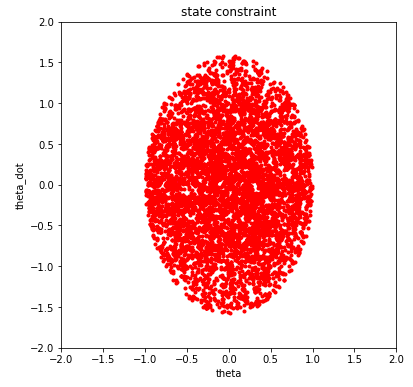
\includegraphics[width=7cm]{region.png}
 	\caption{状態集合$C$}
\end{figure}\\

式$(\ref{CBF})$における$K$を$K(x) = \gamma x$とおくと式(\ref{CBF})は次のようになる.
\begin{equation}
	\sup_{a\in A}\left\{-2\theta\dot{\theta}-\frac{3g\alpha}{l}\dot{\theta}\sin{\theta}-\frac{6\alpha}{ml^2}\dot{\theta} a+\gamma(1-\theta^2-\alpha\dot{\theta}^2)\right\} \geq 0 \label{special_cbf}
\end{equation}
括弧の中は$a$に関する1次式となっているため$\dot{\theta}$の正負に合わせて$U(s)$を定義できる($\frac{6\alpha}{ml^2}$は必ず正のため).\par
さて, 括弧の中身を
\begin{equation}
	p(a) = -2\theta\dot{\theta}-\frac{3g\alpha}{l}\dot{\theta}\sin{\theta}-\frac{6\alpha}{ml^2}\dot{\theta} a+\gamma(1-\theta^2-\alpha\dot{\theta}^2)
\end{equation}
としたとき, $p(a)=0$の解を$a^{*}$とすれば,~$a$は1次元なので$\theta<0$のとき$U(s)$は以下のようになる.
\begin{equation}
	U(s) = 
		\begin{cases}
			[~a^{*}, 10~]~~\textrm{if}~~ a^{*} > -10 \\
			[~-10, 10~]~~\textrm{if}~~ a^{*} \leq -10
		\end{cases}
\end{equation}
また, $\theta>0$のときも同様にすると
\begin{equation}
	U(s) = 
		\begin{cases}
			[~-10, a^{*}~]~~\textrm{if}~~ a^{*} < 10 \\
			[~-10, 10~]~~\textrm{if}~~ a^{*} \geq 10
		\end{cases}
\end{equation}
として与えることができる.

\section{現状}
図2にプロットされている状態$s$に対して, $U(x)$の元を入力しているにもかかわらず, 「シミュレーション上の」次時刻の$h(s_{t+1})$が0よりも小さくなる時があります. \par
その原因を探るべく, 水曜日のzoomでのMTGで, ~$C$内での~$U(x)$をプロットしてみるということも試してみようと話していた(?)ので, 見てみました. \newpage
~
\begin{figure}[h]
	\centering
 	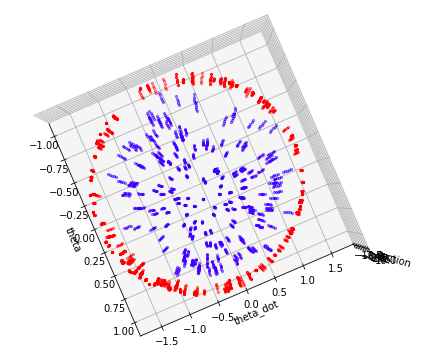
\includegraphics[width=7cm]{theta_thetadot.png}
 	\caption{$\theta, \dot{\theta}$平面への投影}
\end{figure}\\
\begin{figure}[h]
	\centering
 	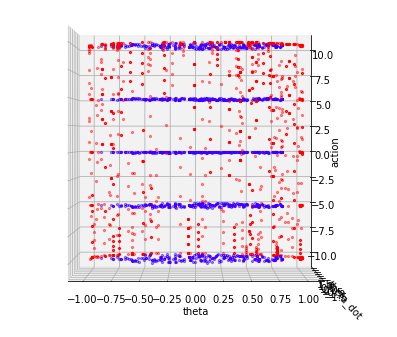
\includegraphics[width=7cm]{theta_action.png}
 	\caption{$\theta, a$平面への投影}
\end{figure}\\
\begin{figure}[h]
	\centering
 	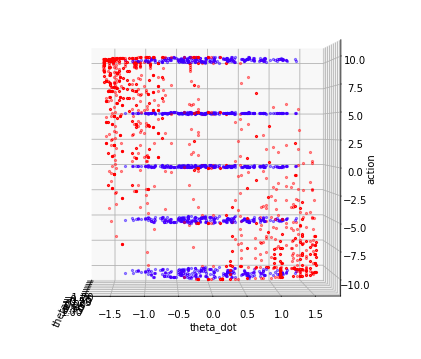
\includegraphics[width=7cm]{thetadot_action.png}
 	\caption{$\dot{\theta}, a$平面への投影}
\end{figure}\par

$C$の要素の$\theta, \dot{\theta}$に対して, $U(s)$の要素を5個づつ等間隔に選び, 3次元空間上にプロットしました. 赤色の点は$C$のフチで, 青色の点は$C$の内部の$\theta, \dot{\theta}$に対する$U(s)$を示しています. 図4を見ると, $\theta$が$-1$に近くても, 負の方向への入力を許していることがわかります. さらに図5を見ると, その場合には$\dot{\theta}$が正方向にあるとわかります. これは直感通り(フチにいても, 逆方向の速度があればOK, という直感)なので, 大まかには$U(s)$を正しく設定できていると思います.\par
なぜそれでも制約が壊れるかを調べるため, $C$のフチの状態$s = [-0.99006819, -0.16353134]$を1つ取ってきて,離散化定数$\delta_t$を変えてシミュレーションしてみました. \par
この時$U(s)$は$[-4.192729709679552, 10.0]$と計算されるため, 入力$a = -4.192729709679552$を加えてみました. 離散化定数$\delta_t=0.05$のときは
\begin{align*}
	s^{\prime} &= [-1.06104261 -1.44708933] \\
	h(x) &= -0.9634384239222334
\end{align*}
となるのに対して, 離散化定数$\delta_t=0.005$のときは
\begin{align*}
	s^{\prime} &= [-0.99015624 -0.17609127] \\
	h(x) &= 0.0071873749226185266
\end{align*}
となり,状態制約を満たします.ここから, 先生のおっしゃっていた通り, 離散化エラーが問題であったことがわかりました. さらに, 離散化定数を限りなく0に近づければ$h(s) = 1- \theta^2- \alpha\dot{\theta}^2$によって安全強化学習できそうだと予測できると思います.

\begin{thebibliography}{10}
\bibitem{event}
D. Baumann, J. J. Zhu, G. Martius, and S. Trimpe. “Deep Reinforcement Learning for Event-Triggered Control."  \textit{In Proc. of the 57th IEEE International Conference on Decision and Control}, 2018.
\bibitem{quad}
Li Wang, Evangelos A Theodorou, and Magnus Egerstedt. “Safe learning of quadrotor dynamics using barrier certificates," \textit{In 2018 IEEE International Conference on Robotics and Automation (ICRA)}, pages 2460-2465, 2018
\bibitem{safe}
R. Cheng, G. Orosz, R. M. Murray, and J. W. Burdick.  “End-to-end safe reinforcement learning through barrier functions for safety-critical continuous control tasks," \textit{Thirty-Third AAAI Conference on Artificial Intelligence}, 2019.

\end{thebibliography}

 
\end{document}